\documentclass[12pt]{article}
 
\usepackage[margin=1in]{geometry} 
\usepackage{amsmath,amsthm,amssymb}
\usepackage{listings}
\usepackage{tikz}
\usepackage{colortbl}
\usepackage{verbatim}
\usetikzlibrary{arrows}

\lstset{basicstyle=\footnotesize}
\usetikzlibrary{calc}

 
\newenvironment{theorem}[2][Theorem]{\begin{trivlist}
\item[\hskip \labelsep {\bfseries #1}\hskip \labelsep {\bfseries #2.}]}{\end{trivlist}}
\newenvironment{lemma}[2][Lemma]{\begin{trivlist}
\item[\hskip \labelsep {\bfseries #1}\hskip \labelsep {\bfseries #2.}]}{\end{trivlist}}
\newenvironment{exercise}[2][Exercise]{\begin{trivlist}
\item[\hskip \labelsep {\bfseries #1}\hskip \labelsep {\bfseries #2.}]}{\end{trivlist}}
\newenvironment{problem}[2][Problem]{\begin{trivlist}
\item[\hskip \labelsep {\bfseries #1}\hskip \labelsep {\bfseries #2.}]}{\end{trivlist}}
\newenvironment{question}[2][Question]{\begin{trivlist}
\item[\hskip \labelsep {\bfseries #1}\hskip \labelsep {\bfseries #2.}]}{\end{trivlist}}
\newenvironment{corollary}[2][Corollary]{\begin{trivlist}
\item[\hskip \labelsep {\bfseries #1}\hskip \labelsep {\bfseries #2.}]}{\end{trivlist}}
\newenvironment{solution}{\begin{proof}[Solution]}{\end{proof}}
 
\begin{document}
 
\title{The Adventure\\
    \large CS120 Problem Solving I}
\author{Harry Coleman}
\date{October 3, 2019}

\maketitle

\section*{Bridge}
\begin{comment}
\fbox{
    \parbox{\textwidth}{
        You only remembered to pack one flashlight, which has a weak beam, so whenever two people cross, they are constrained to walk together, at the speed of the slower person. You can cross the bridge in 5 minutes. Your sister, Maria, can cross it in 10 minutes. Your mom needs 20 minutes, and your father needs 25 minutes. You estimate that you need to get everyone across safely in one hour to escape the wild animals chasing you. Can you do it?
    }
}
\\
\end{comment}

Yes, it is possible to get everyone across within an hour. To show how, we will provide a diagram with the necessary pattern of crossing. First, we will define some symbols for use in the diagram.

\begin{center}
    \begin{tabular}{c|c|c}
         Name & Symbol & Crossing Time(minutes)\\
         \hline
         You & Y & 5\\
         Sister & S & 10\\
         Mom & M & 20\\
         Father & F & 25\\
         Flashlight & (T) & N/A
    \end{tabular}
\end{center}

\begin{center}
    \begin{tabular}{|c|c|c|c|}
        \hline
        \rowcolor[RGB]{200, 200, 200}
        Start & Bridge & End & Times\\
        \hline
        YSMF(T) & & & \\
        \hline
        \rowcolor[RGB]{220, 220, 220}
        MF & YS(T) & & \\
        \rowcolor[RGB]{220, 220, 220}
        MF & $\longrightarrow$ & YS(T) & +10\\
        \hline
        MF & Y(T) & S & \\
        YMF(T) & $\longleftarrow$ & S & +5\\
        \hline
        \rowcolor[RGB]{220, 220, 220}
        Y & MF(T) & S & \\
        \rowcolor[RGB]{220, 220, 220}
        Y & $\longrightarrow$ & SMF(T) & +25\\
        \hline
        Y & S(T) & MF & \\
        YS(T) & $\longleftarrow$ & MF & +10\\
        \hline
        \rowcolor[RGB]{220, 220, 220}
        & YS(T) & MF & \\
        \rowcolor[RGB]{220, 220, 220}
        & $\longrightarrow$ & YSMF(T) &+ 10\\
        \hline
    \end{tabular}
\end{center}

The total time taken here is exactly 60 minutes.

\newpage
\section*{Pills}
Assuming that the pills may be split without losing effectiveness, we would first want to cut each of the three pills in your hand in half. One half of each of the pills can go in a bag to be saved for tomorrow. The other half of each, we will combine with one half of one of the pills in the yellow bottle. In your hand now should be two halves of pills from the blue bottle, and two halves of pills from the yellow bottle. Taking those right now will hopefully yield the same results at one pill from each bottle. The next day, you will have your father take the leftover halves, which should be two halves from the blue bottle, and one half from the yellow bottle. And the other half of the pill from the yellow bottle that you split yesterday. Again, we hope that two half-pills from each bottle yields the same results as one full pill from each bottle. On the remaining two days, your father can take one pill from each bottle as normal.

\section*{Sticks and Rope}


\begin{center}
    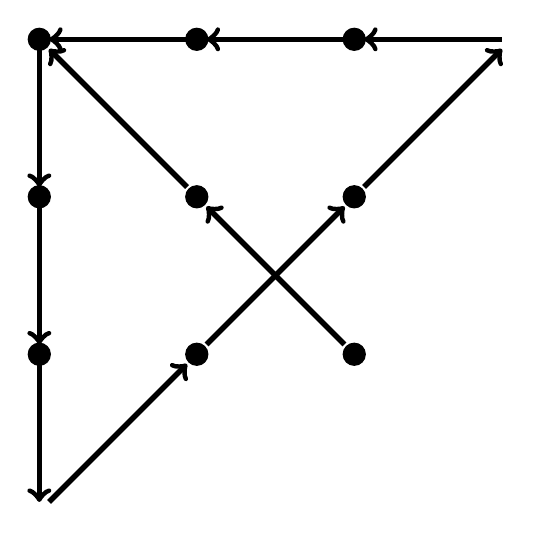
\begin{tikzpicture}[node distance=2cm]
    \node (A) at (0,0) {};
    \node (B) at (2,0) {};
    \node (C) at (4, 0) {};
    \node (D) at (0, -2) {};
    \node (E) at (2, -2) {};
    \node (F) at (4, -2) {};
    \node (G) at (0, -4) {};
    \node (H) at (2, -4) {};
    \node (I) at (4, -4) {};
    \node (J) at (0, -6) {};
    \node (K) at (6, 0) {};
    
    \filldraw[black] (A) circle (4pt);
    \filldraw[black] (B) circle (4pt);
    \filldraw[black] (C) circle (4pt);
    \filldraw[black] (D) circle (4pt);
    \filldraw[black] (E) circle (4pt);
    \filldraw[black] (F) circle (4pt);
    \filldraw[black] (G) circle (4pt);
    \filldraw[black] (H) circle (4pt);
    \filldraw[black] (I) circle (4pt);
    
    \draw [->, line width=2pt]  (I) edge (E)
                                (E) edge (A) 
                                (A) edge (D)
                                (D) edge (G)
                                (G) edge (J)
                                (J) edge (H)
                                (H) edge (F)
                                (F) edge (K)
                                (K) edge (C)
                                (C) edge (B)
                                (B) edge (A);
    \end{tikzpicture}
\end{center}

Pictured above, we start the rope in the lower right, go diagonally to the upper left. Here we make our first bend and go straight down. If we take the distance between each node to be a unit distance, we will go one unit distance below the lower left stick. There, we make our second bend and go diagonally up and right until one unit distance to the right of the upper right stick. The third bend is made here and we go horizontally back to the upper left stick. every time a stick is crossed, the rope is tied and then continues on its path.

\newpage
\section*{Water and Concoction}
We'll represent the proportion of concoction in each bucket with $P_w$ for the water bucket and $P_c$ for the concoction bucket. To start

\[P_w = 0\]
\[P_c = 1\]

Now, we pour a small amount of water $a$ into the concoction bucket. 

\[P_w = 0\]
\[P_c = \frac{1}{1 + a}\]

Notice $P_w$ doesn't change because it is a proportion on concoction, and there is still no concoction in the water bucket. The concoction bucket, on the other hand, has had $a$ water added to the total, thus the denominator increases by $a$. Next, an amount from the concoction bucket is poured back into the water bucket until they have equal volume of liquid. Because $a$ water was poured out of the water bucket, so $a$ liquid needs to be poured back in. The proportion of concoction of the liquid going into the water bucket is $P_c$ because it is from the concoction bucket. So the amount of concoction being added to the water bucket is 

\[a \cdot \frac{1}{1+a} = \frac{a}{1+a}\]

To find the proportion of concoction of water in the water bucket we just take the amount of concoction and divide by the total amount of liquid in the bucket, $1 - a + a = 1$. So

\[P_w = \frac{a}{1+a}\]
\[P_c = \frac{1}{1 + a}\]

So we have the proportions of concoction in each, but we need to find the proportion of foreign liquid. For the water bucket, this is the same value. For the concoction bucket, this is

\[1 - P_c\]
\[1- \frac{1}{1 + a}\]
\[\frac{1+a}{1+a} - \frac{1}{1 + a}\]
\[\frac{a}{1+a}\]

So the amount of foreign liquid in each bucket is the same.

\section*{Rope Escape}
Given that we are able to climb and have a knife, we will assume that you can climb up one rope and reach to cut the other rope, and tie knots while maintaining height. Firstly, you climb up one rope and cut the other rope at the top, while holding onto the cut rope. So you have 50ft of loose rope. Next, move down the rope still attached to the ceiling to about 40ft from the ground and cut it below you, making sure to also hang on to the cut part of the rope. You now have a 50ft piece of rope and a 40ft piece of rope, and you are hanging onto a 10ft rope attached to the ceiling. Near the bottom of the 10ft of rope still remaining, tie a loop with an inner diameter larger than the diameter of the rope. Now, tie the 40ft rope and the 50ft rope together at their ends to create a 90ft piece of rope. Now feed this 90ft rope through the loop in the 10ft rope until on one side hangs 50ft and the other hangs 40ft. Another member of your family on the floor who is heavier than you holds the end of the 50ft end of the rope. You now climb down the 40ft end of the rope to the floor. From the floor, you now pull the 90ft rope all the way out of the loop. Tie this 90ft rope to the hook near the window, climb down 90ft and survive the final 10ft drop.

\newpage
\section*{Card Game}
Taking $n$ to be the number of people playing the game, in this case $n=25$. For all the following, we will assume $n$ to be odd. We will divide the cards into 3 types: low, middle, and high. For an odd $n$ there will be two middle cards, each with the value of $m = (\frac{n-1}{2} +1)$. The low cards will be considered those with a value less than $m$, and high cards those with values greater than $m$. There are the same number of low and high cards, $n-1$. Here is an example of a starting deal with $n=5$, where each column represents a players hand, with the lesser card to be passed on top, and the greater to be held on the bottom.

\begin{center}
    \begin{tabular}{|r|c|c|c|c|c|}
        \hline
        \rowcolor[RGB]{220, 220, 220}
        player & 1 & 2 & 3 & 4 & 5\\
        \hline
        pass & 3 & 1 & 4 & 1 & 2\\
        \hline
        hold & 5 & 2 & 5 & 3 & 4\\
        \hline
    \end{tabular}
\end{center}

If we let one turn play out, the top row will be cycled to the right, with the rightmost card wrapping around to the leftmost slot.

\begin{center}
    \begin{tabular}{|r|c|c|c|c|c|}
        \hline
        \rowcolor[RGB]{220, 220, 220}
        player & 1 & 2 & 3 & 4 & 5\\
        \hline
        pass & 2 & 2 & 1 & 3 & 1\\
        \hline
        hold & 5 & 3 & 5 & 4 & 4\\
        \hline
    \end{tabular}
\end{center}

We can see that in the case of both player 2 and player 4, the new card passed to them was higher than their previously held card, so the new card would be held, and the old card would be passed. 

For a game where $n=5$, $m=3$. So we see that after the first turn, all our low cards are in the pass row, and all our high cards are in the hold row. And our middle cards are one in each row. With and odd $n$ this will always eventually be the case. If given a choice between a low card and a high card, the low card will be passed. And a high card being passed will eventually find a slot in the hold row. Since there are $n$ hold slots, and $n-1$ high cards, every hold slot not occupied by a high card would be a low or middle, and once a high card is passed to that player, it would swap into the hold slot. Therefore all games tend towards all low in pass, all high in hold, and one of each middle in hold and pass. And given that there is one middle being passed around and one middle being held, the two will eventually line up in the same player's hand.



\section*{Light Bulbs}
We will label the switches $A$, $B$, and $C$. You should flip switches $A$ and $B$ to the on position. Wait a few minutes, then flip $B$ to the off position. Now go upstairs to observe the light bulb. If the light bulb is on, then switch $A$ controls the light, since it is the only switch that is flipped on. If the light bulb is off, feel the bulb with your hand. If it is off and warm, then switch $B$ controls the light bulb, because it was turned on, heated up, then turned off and is still warm. If it off and cold, then switch $C$ controls the light bulb because it was never switched on, and thus the light bulb would not have heated up.



\end{document}

